\newpage
\section{System Architecture}
\label{sec:system_architecture}

\subsection{System Components and Key Control Processes}
The distributed cargo approach that we have proposed is dependent on two major innovations. Firstly, the offshore ports are a crucial component of the system. They are intended to be similar in structure to the sort of rigs currently used to extract oil. These ports act as hubs for our second innovation: a large fleet of autonomous shuttle ships. The offshore ports serve as an intermediary between the shuttle ships and pre-existing intercontinental cargo ships. It is the broader distribution of the cargo from these offshore ports that enables greater throughput and efficiency of shipping within a region. As such, the effective allocation and scheduling of autonomous shuttle ships is one of the most important components of the system.

In the proposed system, ports collaborate with shuttle ships in real time to manage the movement of cargo. Offshore ports coordinate the unloading of cargo from conventional intercontinental ships for import to the region served by that particular port. In the simplest terms, cargo from intercontinental ships can be distributed to coastal ports on a first-in-first-out basis, simply summoning shuttle ships as required to transport the cargo to its final destination. The control flow for this process is illustrated in Figure \ref{fig:arch_1}.

\begin{figure}[h!]
\centering
	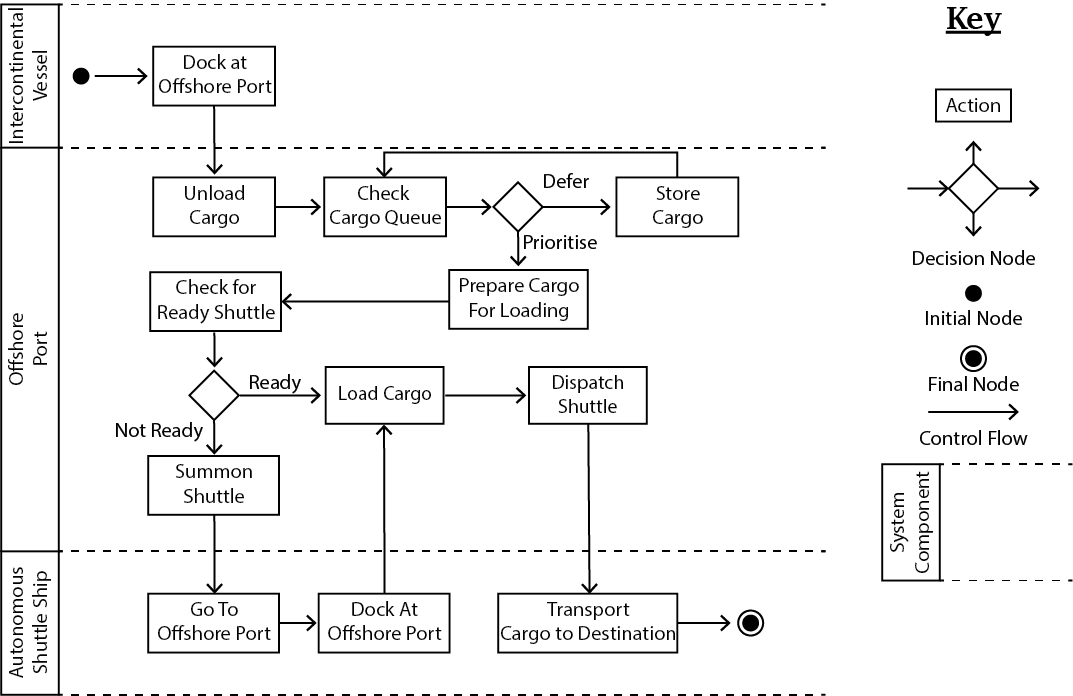
\includegraphics[width=0.85\textwidth]{images/arch_1}
	\caption{Control flow showing the process of transferring inbound cargo at an offshore port from the intercontinental ships to the autonomous shuttle ships.} 
	\label{fig:arch_1}
\end{figure}

Likewise, the ports gather incoming containers from shuttle ships, and route them automatically to intercontinental ships when ready for export. If cargo is not ready for export immediately, it is buffered automatically in a purpose-built container storage system. Since containers in our storage system are not directly stacked, any container in the system can be accessed on demand. The control process for this system is illustrated in Figure \ref{fig:arch_2}.

\begin{figure}[h!]
\centering
	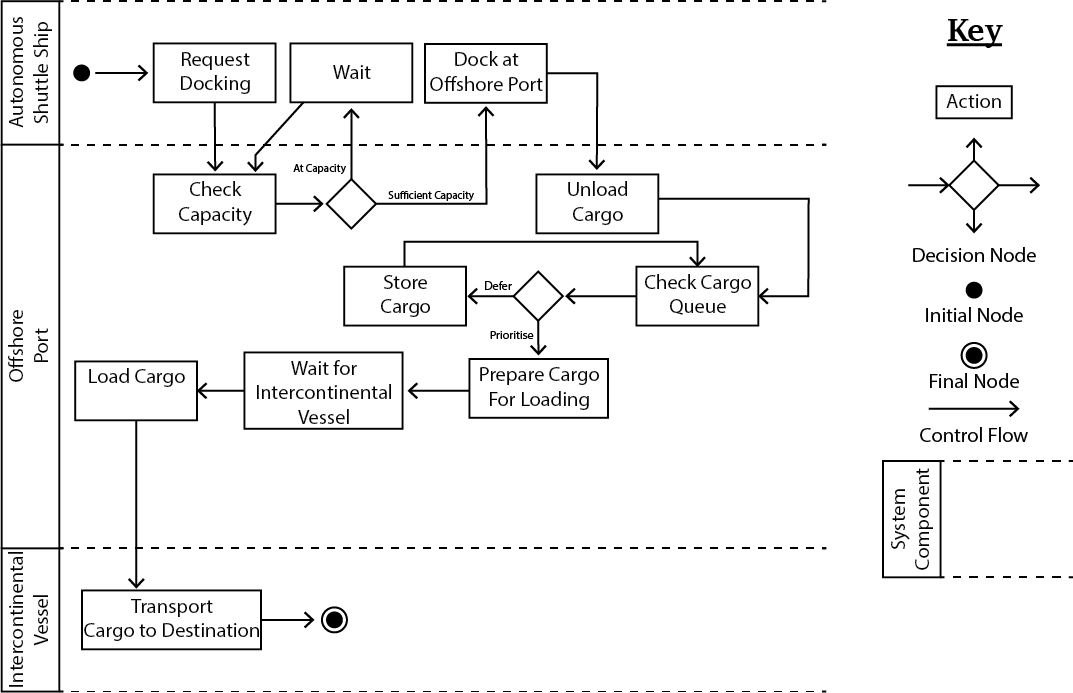
\includegraphics[width=0.85\textwidth]{images/arch_2}
	\caption{Control flow showing the process of transferring outbound cargo at an offshore port from the autonomous shuttle ships to the intercontinental ships.}
	\label{fig:arch_2}
\end{figure}

The size of the shuttle ships is such that each ship will only ever transport cargo to a single destination, rather than offloading subsets at multiple ports. Predictive methods and machine learning will be used to estimate unknown future demand beyond known manifests. We anticipate that this will enhance system efficiency, and reduce the number of required shuttle ships. Such a predictive approach would attempt to prioritise the distribution of cargo so that the amount of cargo stored in offshore ports is minimised. Shuttle ships will give priority to cargo whose destination is a port with a high demand for ships.

Each autonomous shuttle ship acts as an independent autonomous agent. Through a mixture of radar, optical sensors, satellite positioning, and ad-hoc peer-to-peer communication, each ship will independently observe conventional naval navigation rules as a priority. This adherence to the conventions in place today ensures that autonomous shuttle ships can safely cooperate with helmed ships, along with other craft such as leisure vessels. The coordination and communications of vessels is also intended to allow atmospheric conditions to be better accounted for, with the belief that weather fronts can be identified and communicated. Figure \ref{fig:arch_3} shows an overview of the control flow for hazard avoidance used by autonomous shuttle ships.

\begin{figure}[h!]
\centering
	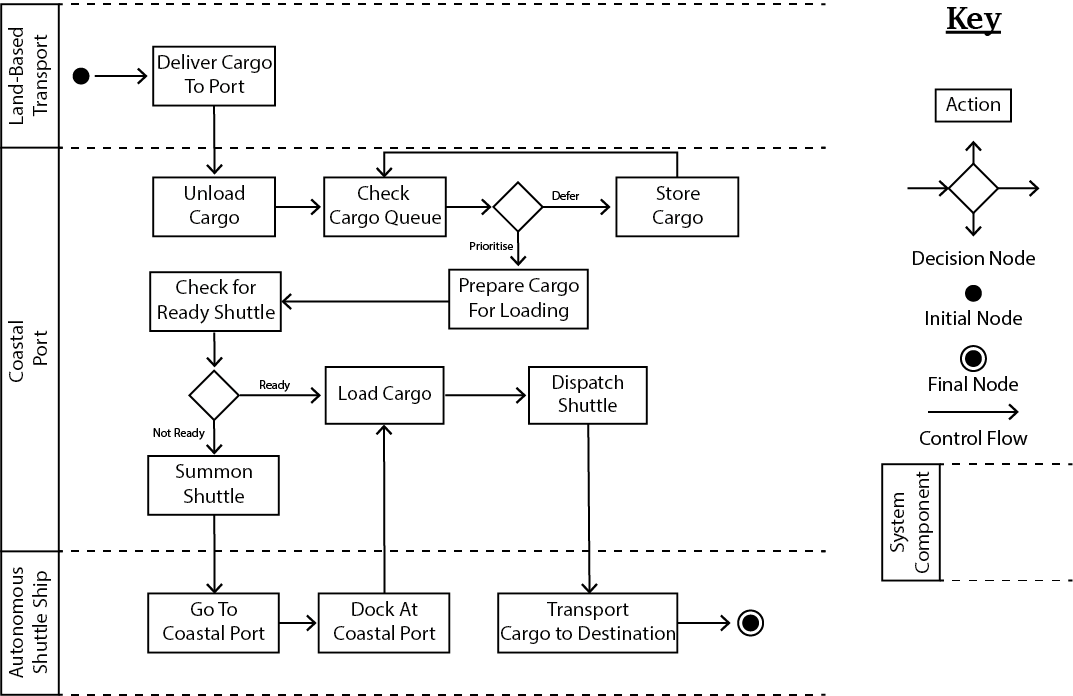
\includegraphics[width=0.85\textwidth]{images/arch_3}
	\caption{Navigation flow showing the process of hazard avoidance by autonomous shuttle ships.}
	\label{fig:arch_3}
\end{figure}

\newpage
\subsection{Use of Assumed Future Capabilities}

The functionality of our system relies on several capabilities that we assume to be feasible in the year 2030. We outlined some of these capabilities in our initial report, but having developed our solution further, we are now in a position to describe how we leverage these capabilities more comprehensively. The majority of our assumptions concern the way in which our offshore ports and shuttle ships will be powered.

Offshore ports would take advantage of nuclear fission to ensure prolonged continuous automated operation. We anticipate that these ports will require large amounts of power. This application of nuclear fission is novel to offshore structures, but draws inspiration from the use of nuclear power in defence submarines. We have also equipped our proposed offshore ports with complex computer vision and robotics systems, driven by neural networks. Between now and 2030, we anticipate significant advances in these areas.

Ports will also be required to service shuttle ships by replenishing their onboard power. This is achieved through a combination of powerful fast wireless charging and a battery swapping system. Both of these systems are not currently fully capable of powering ships, but we anticipate that they will be by the year 2030. We have also assumed that the efficiency of solar panels will have improved substantially by 2030, allowing our shuttle ships to travel long distances.

Finally, the shuttle ships will require an array of sensors and the use of many advanced techniques to ensure safe autonomous operation and navigation. More precise sensory equipment, such as LIDAR, will be required to ensure safe navigation around obstacles when in close proximity. We have taken advantage of anticipated future developments in LIDAR technology to allow our ships to conduct complex manoeuvres, such as docking at offshore ports, with complete autonomy.
